\documentclass[twocolumn,english]{article}
\renewcommand{\familydefault}{\sfdefault}
\usepackage[latin9]{inputenc}
\usepackage[landscape]{geometry}
\geometry{verbose,tmargin=0.5in,bmargin=0.75in,lmargin=0.5in,rmargin=0.5in}
\setlength{\parskip}{0bp}
\setlength{\parindent}{0pt}
\usepackage{float}
\usepackage{booktabs}
\usepackage{amsmath}
\usepackage{graphicx}
\PassOptionsToPackage{normalem}{ulem}
\usepackage{ulem}

\makeatletter

\providecommand{\tabularnewline}{\\}




\PassOptionsToPackage{normalem}{ulem}




\providecommand{\tabularnewline}{\\}




\PassOptionsToPackage{normalem}{ulem}




\providecommand{\tabularnewline}{\\}




\usepackage{array}
\usepackage{multirow}






\providecommand{\tabularnewline}{\\}

\setlength{\columnsep}{0.25in}
\usepackage{xcolor}
\usepackage{textcomp}
\usepackage{listings}
\lstset{
  tabsize=2,
  basicstyle=\small\ttfamily,
}



\usepackage{babel}
\usepackage{listings}
\renewcommand{\lstlistingname}{Listing}



\usepackage{titlesec}
\titleformat*{\section}{\color{blue!60!green!40!black} \vspace{8pt}\titlerule\vspace{4pt}\Large\bfseries\sffamily}
\titleformat*{\subsection}{\color{blue!60!green} \vspace{2pt}\large\bfseries\sffamily}



\usepackage{enumitem}
\setlist{itemsep=0pt}


\let\emph\relax
\DeclareTextFontCommand{\emph}{\bfseries}



\usepackage{babel}




\usepackage{babel}
\usepackage{listings}
\renewcommand{\lstlistingname}{Listing}

\makeatother

\usepackage{babel}
\usepackage{listings}
\renewcommand{\lstlistingname}{Listing}

\begin{document}

\title{\vspace{-4ex}
 Revision Notes for CO221 Compilers\vspace{-4ex}
 }

\date{Autumn 2017\vspace{-2ex}
 }

\maketitle
\begin{figure}[H]
\centering{}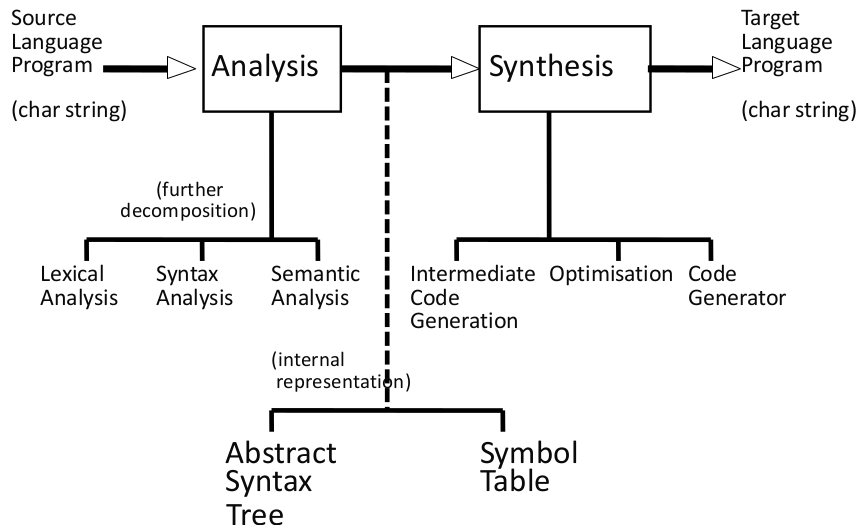
\includegraphics[width=0.7\linewidth]{img/compiler} 
\end{figure}

\section{Lexical Analysis}

Transforms a stream of characters into tokens.

\subsection{Tokens}

\paragraph{Identifier Tokens}
\begin{itemize}
\item \emph{Keyword identifiers}, e.g. \texttt{while} - generally have their
own token. 
\item \emph{Non-keyword identifiers} - have a general identifier token e.g.
\texttt{IDENT(\char`\"{}year\char`\"{})}. 
\end{itemize}
Use a fast lookup function to determine if a scanned identifier is
a keyword (e.g. perfect hash).

\paragraph{Literal Tokens}
\begin{itemize}
\item \emph{Unsigned integers} - represented by a token for integers, plus
an integer. 
\item \emph{Unsigned reals}, \emph{strings} represented similarly. 
\end{itemize}

\paragraph{Other Tokens}
\begin{itemize}
\item \emph{1 or 2-char symbols}, e.g. +, \textless{}= usually represented
by their own token. 
\item \emph{Whitespace} and \emph{comments} usually not represented in token
stream. 
\item \emph{Macros} usually removed before lexical analysis. 
\end{itemize}

\subsection{Regular Expressions}
\begin{enumerate}
\item Write \emph{test cases}. 
\item Re-cast the question using standard characters instead of meta-characters. 
\item Try drawing a DFA if easier. 
\end{enumerate}
\begin{table}[H]
\centering{}%
\begin{tabular}{cc}
\toprule 
 & \textbf{\footnotesize{}{}{}Matches}\tabularnewline
\midrule 
\texttt{a}  & {\footnotesize{}{}{}Symbol}\tabularnewline
$\epsilon$  & {\footnotesize{}{}{}Empty string}\tabularnewline
\texttt{R1 R2}  & \texttt{\footnotesize{}{}{}R1}{\footnotesize{}{}{} followed by
}\texttt{\footnotesize{}{}{}R2}\tabularnewline
\texttt{R1\textbar{}R2}  & \texttt{\footnotesize{}{}{}R1}{\footnotesize{}{}{} or }\texttt{\footnotesize{}{}{}R2}\tabularnewline
\texttt{R{*}}  & {\footnotesize{}{}{}0 or more occurrence of }\texttt{\footnotesize{}{}{}R}\tabularnewline
\texttt{(R)}  & \texttt{\footnotesize{}{}{}R}\tabularnewline
\texttt{\textbackslash{}a}  & {\footnotesize{}{}{}Escaped symbol}\tabularnewline
\midrule 
\texttt{R?}  & {\footnotesize{}{}{}0 or 1 occurrence of }\texttt{\footnotesize{}{}{}R}\tabularnewline
\texttt{R+}  & {\footnotesize{}{}{}1 or more occurrence of }\texttt{\footnotesize{}{}{}R}\tabularnewline
\texttt{{[}a-zA-Z{]}}  & {\footnotesize{}{}{}Any character from given set}\tabularnewline
\texttt{{[}\textasciicircum{}a-zA-Z{]}}  & {\footnotesize{}{}{}Any character except from given set}\tabularnewline
\texttt{.}  & {\footnotesize{}{}{}Any character except newline}\tabularnewline
\bottomrule
\end{tabular}
\end{table}

\subsection{Rules}

\paragraph{Regular Expression Rules}

\emph{Rules} (\emph{productions}) of the form $\alpha\rightarrow\texttt{X}$
where $\alpha$ is a \emph{non-terminal} (name of rule) and \texttt{X}
is a regular expression constructed from both non-terminals and terminals
(input chars).

\emph{Note} that non-terminals must be defined before use, and recursion
is not allowed.

E.g. 
\begin{itemize}
\item $\texttt{Digit}\rightarrow\texttt{[0-9]}$ 
\item $\texttt{Int}\rightarrow\texttt{Digit+}$ 
\end{itemize}

\paragraph{Disambiguation Rules}
\begin{enumerate}
\item Use \emph{longest matching character sequence}. 
\item Assume regular expressions have \emph{textual precedence} (earliest
matching regular expression chosen). 
\end{enumerate}

\paragraph{Implementation}

Either hand-crafted, or use lexical analyser generator (e.g. Flex).

\begin{figure}[H]
\begin{centering}
\emph{Lexical analyser generator}: 
\par\end{centering}
\centering{}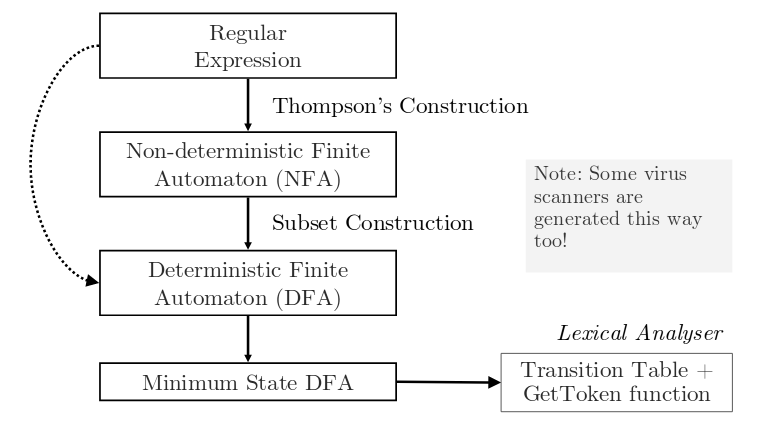
\includegraphics[width=0.75\linewidth]{img/lex} 
\end{figure}

\subsection{Finite Automata}
\begin{itemize}
\item \emph{States} of matching process (circles). 
\item \emph{Transitions} between those states (arrows). 
\item Matched input \emph{symbols} (labels on transitions). 
\item \emph{Accepting states} of matching process (double circle). 
\item \emph{Start state} (unlabelled incoming arrow). 
\end{itemize}

\paragraph{Deterministic Finite Automata}

No two transitions leaving a state have the same symbol.

\paragraph{Non-deterministic Finite Automata}

Allow a choice of transitions out of a state

\paragraph{Thompson's Construction}

Use $\epsilon$ transitions to glue together automata for each part
of a regex:

\begin{figure}[H]
\begin{centering}
\texttt{r1 r2} 
\par\end{centering}
\centering{}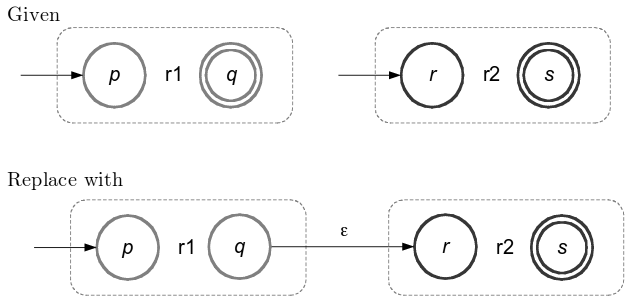
\includegraphics[width=0.5\linewidth]{img/concat} 
\end{figure}

\begin{figure}[H]
\begin{centering}
\texttt{r1\textbar{}r2} 
\par\end{centering}
\centering{}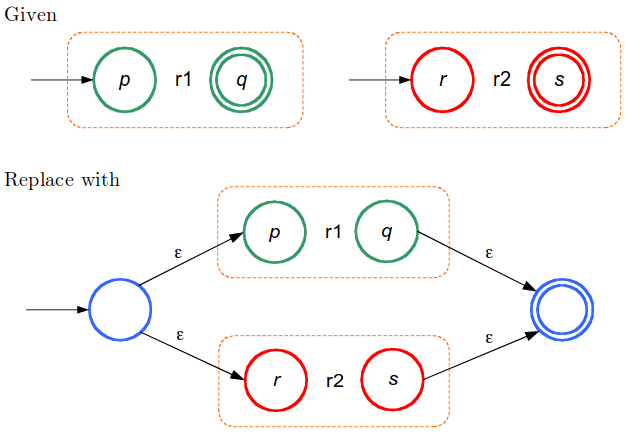
\includegraphics[width=0.5\linewidth]{img/alternate} 
\end{figure}

\begin{figure}[H]
\begin{centering}
\texttt{r1{*}} 
\par\end{centering}
\centering{}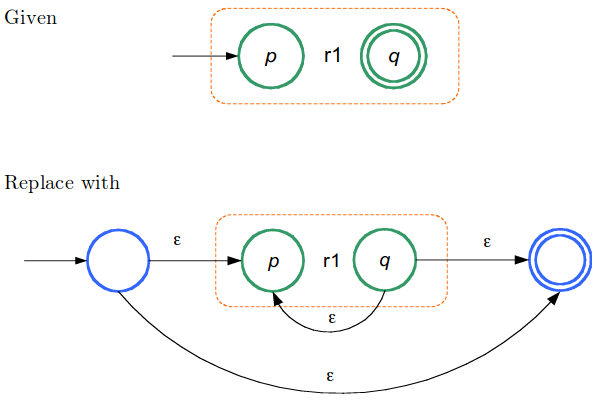
\includegraphics[width=0.5\linewidth]{img/repeat} 
\end{figure}

\paragraph{Subset Construction}
\begin{itemize}
\item DFAs are much faster than NFAs (linear on size of input string), 
\item but require more memory (potentially $2^{n}$ states for an $n$-state
NFA). 
\end{itemize}
\emph{Algorithm}: 
\begin{enumerate}
\item DFA start state = $\epsilon$ closure of NFA start state. 
\item For each new subset state $S$ of the DFA:
\begin{enumerate}
\item For each unique symbol \texttt{a} leading out from any state of $S$:
\begin{enumerate}
\item Add a transition \texttt{a} from S to S' where S' = $\epsilon$ closure
of states reached by \texttt{a} 
\end{enumerate}
\end{enumerate}
\end{enumerate}

\paragraph{Generating a Lexical Analyser}

Encode DFA as a 2D table of states (row per state, col per char).

\section{Parsing}

Transforms a stream of tokens to an AST based on context free grammar
of the language.

\subsection{LR (Bottom-Up / Shift-Reduce) Parsing}
\begin{itemize}
\item Can be implemented in $O(n)$ time. 
\item Several methods for generating LR parsing tables. States consist of
LR(k) items of the grammar, vary in number of states and size of lookahead
sets. 
\end{itemize}

\paragraph{Context Free Grammars}

Test very carefully.

\subsubsection{LR(0) Parsing}

Don't use the current token in order to perform a reduce. E.g the
rule $\texttt{X}\rightarrow\texttt{ABC}$ has 4 LR(0) items, where
$\bullet$ indicates how much of the rule we have seen: 
\begin{enumerate}
\item $\texttt{X}\rightarrow\texttt{\ensuremath{\bullet}ABC}$ 
\item $\texttt{X}\rightarrow\texttt{A\ensuremath{\bullet}BC}$ 
\item $\texttt{X}\rightarrow\texttt{AB\ensuremath{\bullet}C}$ 
\item $\texttt{X}\rightarrow\texttt{ABC\ensuremath{\bullet}}$ 
\end{enumerate}

\paragraph{LR(0) to Finite Automata}
\begin{enumerate}
\item Add a start rule with end-of-input symbol: e.g. $\texttt{E'}\rightarrow\texttt{E}\texttt{\$}$. 
\item For each LR(0) item: 
\end{enumerate}
Given $\texttt{X}\rightarrow\texttt{A\ensuremath{\bullet}BC}$, we
add the transition:

\begin{figure}[H]
\centering{}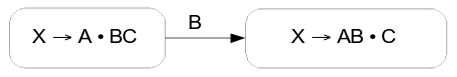
\includegraphics[width=0.4\linewidth]{img/lr0tonfa} 
\end{figure}

Suppose \texttt{B} is a non-terminal, then for all $\texttt{B}\rightarrow\texttt{\ensuremath{\bullet}D}$,
we add $\epsilon$ transitions of the form:

\begin{figure}[H]
\centering{}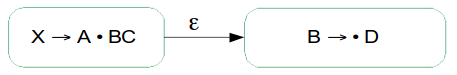
\includegraphics[width=0.4\linewidth]{img/lr0tonfa-nonterminal} 
\end{figure}

We then construct a DFA using subset construction. 
\begin{enumerate}
\item Usually it's simple to construct the DFA directly. 
\item Try and keep the DFA neat - otherwise it's easy to get lost. 
\item Check very carefully for duplicate states. 
\end{enumerate}

\paragraph{Finite Automata to Parsing Table}
\begin{enumerate}
\item For each terminal transition $\texttt{X}\xrightarrow{\texttt{T}}\texttt{Y}$,
add $\texttt{P}[\texttt{X},\texttt{T}]=s\texttt{Y}$ (\textbf{shift}
\texttt{Y}). 
\item For each non-terminal transition $\texttt{X}\xrightarrow{\texttt{N}}\texttt{Y}$,
add $\texttt{P}[\texttt{X},\texttt{N}]=g\texttt{Y}$ (\textbf{goto}
\texttt{Y}). 
\item For each state \texttt{X} containing the item $\texttt{R'}\rightarrow\dots\bullet$,
add $\texttt{P}[\texttt{X},\texttt{\$}]=a$ (\textbf{accept}). 
\item For each state \texttt{X} containing the item $\texttt{R}\rightarrow\dots\bullet$,
add $\texttt{P}[\texttt{X},\texttt{T}]=rN$ (\textbf{reduce}), for
every terminal \texttt{T} where $N$ is $R$'s rule number. 
\end{enumerate}

\paragraph{Model of an LR Parser}

Modelled by pushdown automata: 
\begin{itemize}
\item \emph{Shift} pushes state onto stack and advances token. 
\item \emph{Reduce}:
\begin{itemize}
\item removes $L$ tokens from the stack ($L$ is the length of the RHS
of the rule), 
\item pushes the state of the \emph{goto} for the LHS of the rule according
to the state now on the top of the stack, 
\item and generates an AST node for the rule. 
\end{itemize}
\end{itemize}

\subsubsection{Other LR Parsing Methods}
\begin{itemize}
\item \emph{FIRST set} for a sequence of non-terminals and terminals $\alpha$
is the set of all tokens that could start a derivation of $\alpha$,
including $\epsilon$ if $\alpha$ can derive $\epsilon$.
\begin{itemize}
\item A non-terminal \texttt{A} is \emph{nullable} if $A\implies^{*}\epsilon$. 
\end{itemize}
\item \emph{FOLLOW set} for a non-terminal \texttt{A} is the set of all
tokens that could immediately follow \texttt{A}, including \texttt{\$}
if \texttt{A} can end the input. I.e. For each derivation of $\texttt{X}\rightarrow\texttt{ABC}$:
\begin{enumerate}
\item \texttt{FOLLOW(B)} includes \texttt{FIRST(C)}. 
\item If \texttt{FIRST(C)} includes $\epsilon$, then \texttt{FOLLOW(B)}
includes \texttt{FOLLOW(X)}. 
\item If \texttt{C} is empty, then \texttt{FOLLOW(B)} includes \texttt{FOLLOW(X)}. 
\end{enumerate}
\end{itemize}
Check FOLLOW sets very carefully, and pay special attention to rules
with $\epsilon$ in their FIRST set.

\paragraph{Different LR Parsers}
\begin{itemize}
\item LR(0): A reduce item $\texttt{X}\rightarrow\texttt{A\ensuremath{\bullet}}$
always causes a reduction. 
\item SLR(1): A reduce item $\texttt{X}\rightarrow\texttt{A\ensuremath{\bullet}}$
causes a reduction only if the current token is in FOLLOW(\texttt{X}). 
\item LR(1): A reduce item $\texttt{X}\rightarrow\texttt{A\ensuremath{\bullet}},\texttt{t}$
causes a reduction only if the current token is \texttt{t}.
\begin{itemize}
\item \emph{FA Transitions}: For each rule $\texttt{X}\rightarrow\texttt{A\ensuremath{\bullet}BC},\texttt{t}$:
\begin{itemize}
\item Add transition via \texttt{B} to $\texttt{X}\rightarrow\texttt{AB\ensuremath{\bullet}C},\texttt{t}$. 
\item For each rule $\texttt{B}\rightarrow\texttt{D}$ and every token \texttt{u}
in \texttt{FIRST(Ct)}, add transitions via $\epsilon$ to $\texttt{B}\rightarrow\texttt{D},\texttt{u}$. 
\end{itemize}
\end{itemize}
\item LALR(1): Combines LR(1) states that differ in the look-ahead token
only. This can cause spurious reductions before an error is detected. 
\end{itemize}

\subsubsection{Ambiguities}

Grammars which can derive more than 1 parse tree for some input cannot
be LR($k$) for any $k$.

\paragraph{Shift-Reduce Conflicts}

Usually obvious in a DFA. E.g. Consider the grammar:

\begin{alignat*}{2}
\texttt{S} & \rightarrow & if\texttt{ E }then\texttt{ S }else\texttt{ S}\\
\texttt{S} & \rightarrow & if\texttt{ E }then\texttt{ S}\\
\texttt{S} & \rightarrow & id\\
\texttt{E} & \rightarrow & 0\mid1
\end{alignat*}

and the statement: 
\[
if\texttt{ a }then\texttt{ }if\texttt{ b }then\texttt{ c }else\texttt{ d}
\]
\begin{itemize}
\item If we shift first, we get: $if\texttt{ a }then\texttt{ }\boxed{if\texttt{ b }then\texttt{ c }else\texttt{ d}}$. 
\item If we reduce first, we get: $if\texttt{ a }then\texttt{ }\boxed{if\texttt{ b }then\texttt{ c}}\texttt{ }else\texttt{ d}$. 
\end{itemize}
\emph{Solution}: rewrite the grammar: 
\begin{align*}
\texttt{S} & \rightarrow & \texttt{MatchedS}\\
\texttt{MatchedS} & \rightarrow & if\texttt{ E }then\texttt{ MatchedS }else\texttt{ MatchedS}\\
\texttt{MatchedS} & \rightarrow & id
\end{align*}
\begin{align*}
\texttt{S} & \rightarrow & \texttt{UnmatchedS}\\
\texttt{UnmatchedS} & \rightarrow & if\texttt{ E }then\texttt{ S}\\
\texttt{UnmatchedS} & \rightarrow & if\texttt{ E }then\texttt{ MatchedS }else\texttt{ UnmatchedS}
\end{align*}

We now force $else$-parts to become matched as soon as possible.

\paragraph{Reduce-Reduce Conflicts}

Can usually tell from ambiguities. Consider the grammar: 
\[
\texttt{Expr}\rightarrow\texttt{Expr `+' Expr}\mid\texttt{Expr `*' Expr}\mid\texttt{`(' Expr `)'}\mid int
\]

This is ambiguous because it doesn't define the associativity or precedence
of \texttt{+} and \texttt{{*}}.

\emph{Solution}: rewrite the grammar: 
\begin{align*}
\texttt{Expr} & \rightarrow & \texttt{Expr `+' Term}\mid\texttt{Term}\\
\texttt{Term} & \rightarrow & \texttt{Term `*' Factor}\mid\texttt{Factor}\\
\texttt{Factor} & \rightarrow & \texttt{`(' Expr `)'}\mid int
\end{align*}

\paragraph{Parse Trees}
\begin{enumerate}
\item \emph{Naranker}: build leaf nodes for each input token (\emph{shift})
and non-leaf nodes for each rule (\emph{reduce}). 
\item \emph{Paul}: one branch for every item on the RHS of a rule. 
\end{enumerate}

\paragraph{Abstract Syntax Trees}

Remove unnecessary information from the parse tree - can be constructed
by a separate parse or by attaching AST construction code directly
to grammar rules.

\subsection{LL (Top-Down) Parsing}

A language is LL($k$) if $k$-token lookahead is sufficient to choose
between alternatives of a rule when parsing.

\paragraph{Backus-Naur Form (BNF)}

The rules for a CFG take the form $\texttt{A}\rightarrow\alpha$ where
\texttt{A} is a rule and $\alpha$ is a possibly empty sequence of
rules and tokens.

\paragraph{Extended BNF (EBNF)}
\begin{itemize}
\item $\left\{ \alpha\right\} $: 0 or more occurrences of $\alpha$. (\emph{Repetition})
\begin{itemize}
\item $\left\{ \texttt{E}\right\} $ becomes $\texttt{X}\rightarrow\epsilon\mid\texttt{XE}$ 
\end{itemize}
\item $\left[\alpha\right]$: 0 or 1 occurrence of $\alpha$. (\emph{Optional})
\begin{itemize}
\item $\left[\texttt{E}\right]$ becomes $\texttt{X}\rightarrow\epsilon\mid\texttt{E}$ 
\end{itemize}
\item $\left(\alpha\right)$: $\alpha$. (\emph{Grouping}) 
\end{itemize}

\paragraph{LL(1)}

A grammar is LL(1) if it: 
\begin{enumerate}
\item For each distinct pair of alternatives $(\alpha,\beta)$ of a rule
\texttt{A}, FIRST($\alpha$) and FIRST($\beta$) are disjoint. 
\item For every rule \texttt{A}, if FIRST(\texttt{A}) contains $\epsilon$,
then FIRST(\texttt{A}) and FOLLOW(\texttt{A}) are disjoint. 
\end{enumerate}

\paragraph{Recursive Descent Parser}

Consists of: 
\begin{itemize}
\item Set of \emph{parse functions}, one for each rule (which returns AST
for the rule). E.g. 
\begin{lstlisting}[tabsize=4]
def BeginStatement():
	match(BEGIN)
	statlist = []
	statlist.append(Statement())
	while token == SEMICOLON:
		match(SEMICOLON)
		statlist.append(Statement())
	match(END)
	return BeginAST(statList)
\end{lstlisting}
\item The current \emph{input token}, e.g. as a variable. 
\item A token \emph{match} and advance function. 
\begin{lstlisting}[tabsize=4]
def match():
	if token == expected:
		token = scanner.get_token()
	else error ("unexpected token...")
\end{lstlisting}
\end{itemize}

\paragraph{CFG to LL(1)}

3 common transformations: 
\begin{enumerate}
\item \emph{Left recursion removal}: E.g.
\begin{enumerate}
\item $\texttt{A}\rightarrow\texttt{X}\mid\texttt{AY}$ is rewritten as
$\texttt{A}\rightarrow\texttt{X}\left\{ \texttt{Y}\right\} $. 
\end{enumerate}
\item \emph{Substitution}: Replace non-terminal \texttt{A} on LHS of a rule
with each of the alternatives of \texttt{A}. 
\item \emph{Left factorisation}: E.g.
\begin{enumerate}
\item $\texttt{A}\rightarrow\texttt{BC}\mid\texttt{BD}$ is rewritten as
$\texttt{A}\rightarrow\texttt{B}\left(\texttt{C}\mid\texttt{D}\right)$. 
\item $\texttt{A}\rightarrow\texttt{BC}\mid\texttt{B}$ is rewritten as
$\texttt{A}\rightarrow\texttt{B}\left[\texttt{C}\right]$. 
\end{enumerate}
\end{enumerate}

\paragraph{Error Recovery}

We try to: 
\begin{enumerate}
\item Produce informative messages, 
\item If recovery is attempted, skip as little as possible, 
\item If correction is attempted, ensure corrected program has same syntax
tree and semantics as original. 
\end{enumerate}
In panic mode error recovery: 
\begin{itemize}
\item Each parse function has a set of synchronising tokens (\emph{syncset}).
E.g. 
\begin{lstlisting}[tabsize=4]
def IfStatement(syncset):
	match(IF)
	Expr(syncset union {THEN, ELSE})
	match(THEN)
	Statement(syncset union {ELSE})
	check({ELSE}, syncset, "Error ...")
	if token  ==  ELSE:
		match(ELSE)
		Statement(syncset)
\end{lstlisting}
\item When an error occurs, we skip ahead, discarding tokens until one of
the synchronising tokens is seen. 
\begin{lstlisting}[tabsize=4]
def check(expectset, syncset, message):
	if token not in expectset:
		error(message)
		while token not in (expectset union syncset)
		      and token != EOF:
			scanner .get_token() # skip tokens
\end{lstlisting}
\end{itemize}

\section{Semantic Checking}

We can check for errors during \emph{parsing}, \emph{semantic checking}
(i.e. with a symbol table), and at \emph{runtime}. Sometimes we \emph{ignore}
them (e.g. integer overflow, infinite loops).

\paragraph{Type Checking in Languages}

Can vary greatly. Languages may support: 
\begin{itemize}
\item No explicitly typed variables (types inferred). 
\item Dynamically typed variables (types can change). 
\item Overloaded functions and polymorphic typing. 
\item Non-standard assignment-compatibility / type equivalence. 
\item Restrictions on how some types are used. 
\item Implicit type casting. 
\item Identifiers being used to name several kinds of entities. 
\item Multiple sizes for integers and floats. 
\end{itemize}

\paragraph{Symbol Tables}

A dictionary from identifiers to AST nodes or objects holding identifier
information. Standard implementation: 
\begin{itemize}
\item \emph{Top-level symbol table} pre-loaded with identifier entries for
globally visible identifiers, e.g. standard types, constants, functions... 
\item New symbol table for each scope, with dictionaries from identifiers
to types. 
\end{itemize}

\subsection{Example Checks}

\paragraph{Variable Declaration}
\begin{enumerate}
\item Check that the identifier is in scope. 
\item Check type is valid, and objects of this type can be declared. 
\item Check identifier isn't already defined. 
\item Add variable to symbol table. 
\end{enumerate}
\begin{figure}[H]
\centering{}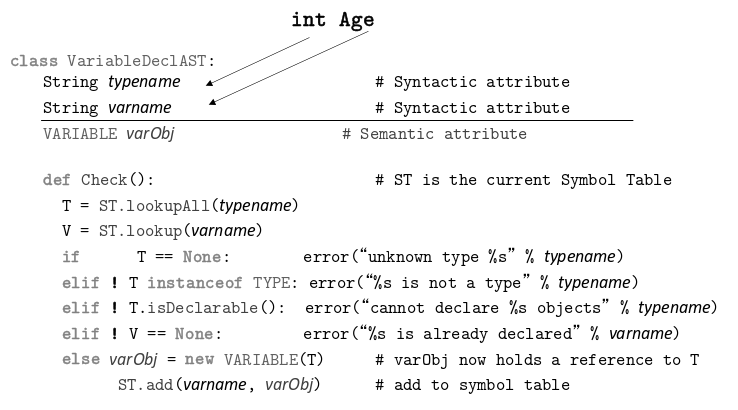
\includegraphics[width=0.8\linewidth]{img/var-declaration} 
\end{figure}

\paragraph{Assignment}
\begin{enumerate}
\item Check identifier is in scope and is a variable. 
\item Check the types are compatible. 
\end{enumerate}
\begin{figure}[H]
\centering{}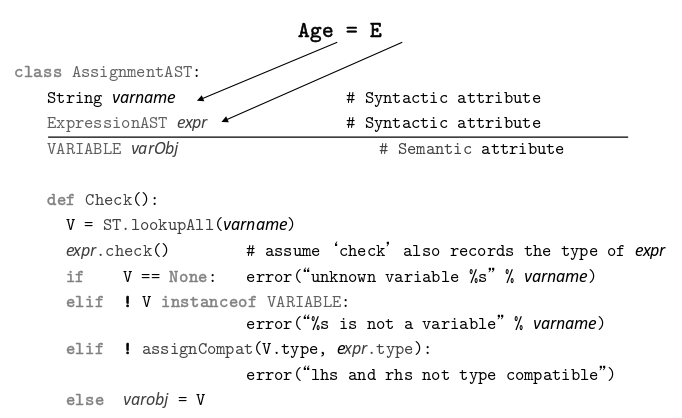
\includegraphics[width=0.75\linewidth]{img/assignment} 
\end{figure}

\paragraph{Function Declaration}
\begin{enumerate}
\item Check return type is valid, and objects of this type can be returned. 
\item Check the function isn't already defined. 
\item Add function to the symbol table. 
\item Create and link new symbol table. 
\item Check parameter declarations. 
\end{enumerate}
\begin{figure}[H]
\centering{}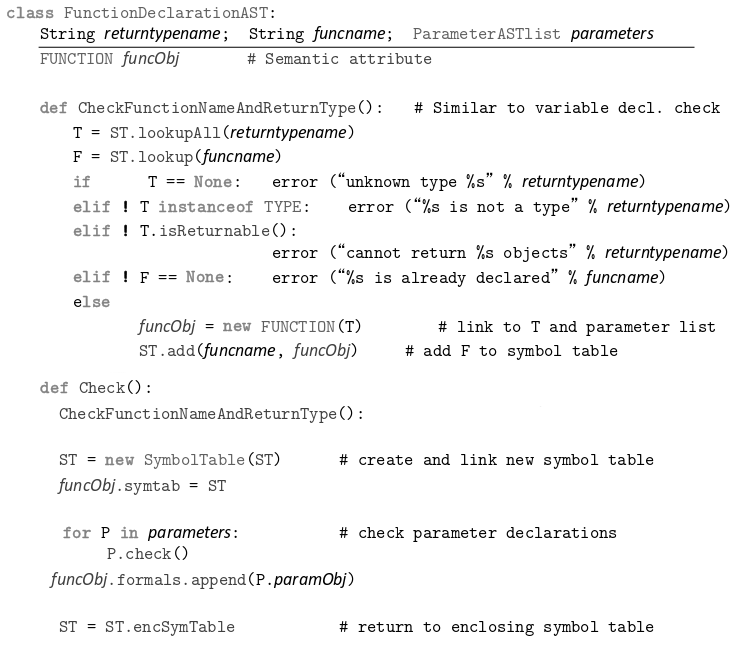
\includegraphics[width=0.8\linewidth]{img/func-declaration} 
\end{figure}

\paragraph{Function Call}
\begin{enumerate}
\item Check function exists. 
\item Check length of parameters. 
\item Check parameters. 
\item Check return type. 
\end{enumerate}
\begin{figure}[H]
\centering{}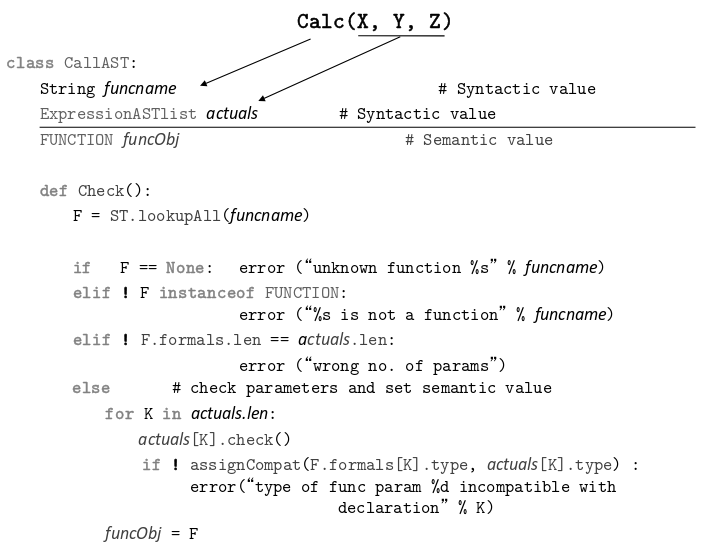
\includegraphics[width=0.75\linewidth]{img/func-call} 
\end{figure}

\section{Runtime Memory Organisation}

\subsubsection*{Basic Types}
\begin{itemize}
\item \emph{Primitive types}: mapped to memory locations and/or registers.
Sometimes memory aligned to keep accesses optimal. 
\item \emph{Records} / \emph{structures}: fields are grouped together and
usually allocated consecutively in memory. Fields accessed by a constant
byte offset from start. 
\item \emph{Arrays}: variables of same size grouped together and accessed
by a runtime integer expression that gives the offset from the start. 
\end{itemize}

\subsubsection*{Objects}
\begin{itemize}
\item \emph{Fields}: memory location of object reference + offset of field. 
\item \emph{Methods}: object reference passed as a hidden parameter. 
\item \emph{Inheritance}, \emph{overriding} and \emph{dynamic binding}:
\begin{figure}[H]
\centering{}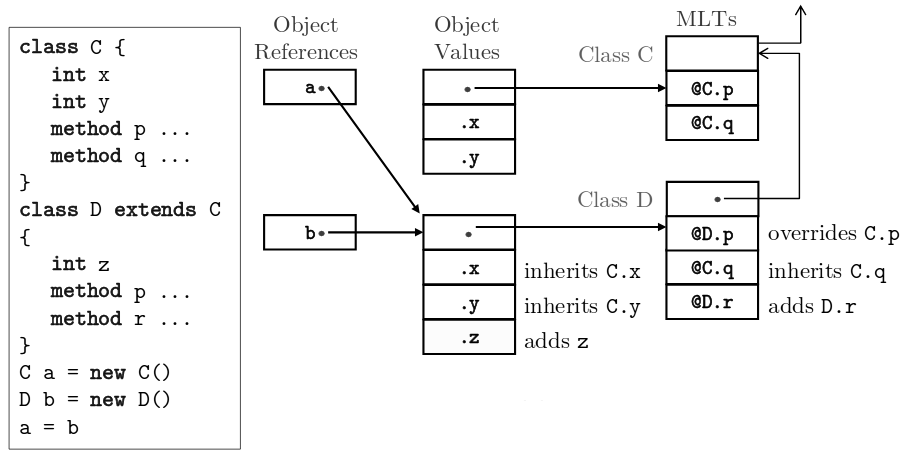
\includegraphics[width=0.75\linewidth]{img/objects} 
\end{figure}
\end{itemize}

\paragraph{Program Address Space}
\begin{itemize}
\item \emph{Code segment}. 
\item \emph{Stack segment}: for storing local variables.
\begin{itemize}
\item Access is through the \emph{frame pointer register}. 
\item For \emph{method calls}: we also hold the return address, address
of the method's of object, parameters, saved values of registers,
space for a return value. 
\begin{figure}[H]
\centering{}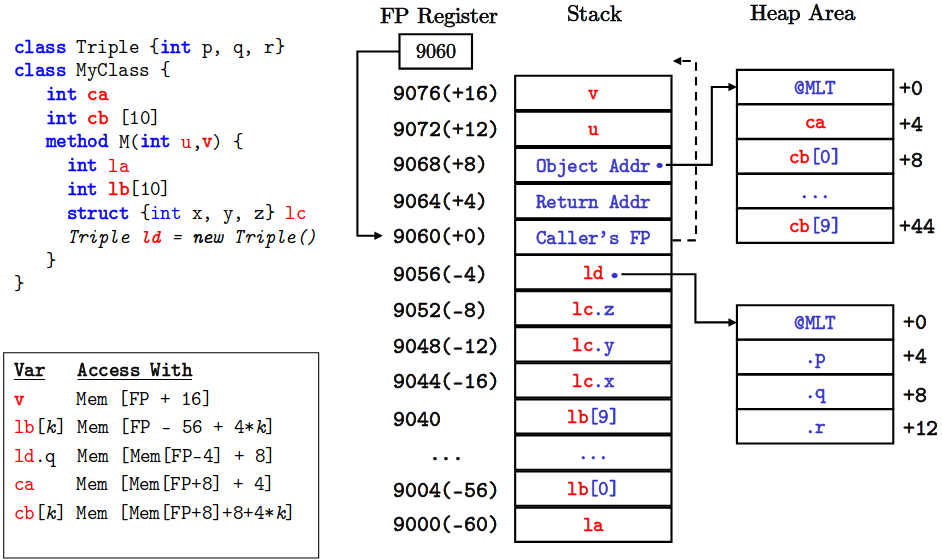
\includegraphics[width=0.75\linewidth]{img/stack} 
\end{figure}
\end{itemize}
\item \emph{Data segment}.
\begin{itemize}
\item \emph{Static area}: for storing global / static variables (also constants
and MLTs sometimes). 
\item \emph{Heap area}.
\begin{itemize}
\item Keep a \emph{FreeList} (chain of pointers to unused / returned / garbage
collected memory blocks in the heap area). 
\item Maintain different free lists for different block-size intervals. 
\end{itemize}
\end{itemize}
\end{itemize}

\paragraph{Garbage Collection}

The garbage collector needs to know: 
\begin{itemize}
\item Which variables in the program point to the heap. 
\item For each object pointed to, which pointers it contains. 
\end{itemize}
\emph{Heap compaction}: Reduce fragmentation by: 
\begin{enumerate}
\item Mark live blocks. 
\item Co-locate live blocks. 
\item Update the pointers that point to co-located blocks. 
\end{enumerate}
Algorithms include: 
\begin{enumerate}
\item \textbf{Reference-Counting.} Record in each block the number of pointers
that point to the block.
\begin{itemize}
\item Needs techniques to reclaim cyclic data structures. 
\end{itemize}
\item \textbf{Mark-Sweep.} Has two phases:
\begin{enumerate}
\item \emph{Mark phase}: mark all blocks that are reachable from non-heap
references. 
\item \emph{Sweep phase}: scan all blocks, reclaiming dead blocks and unmarking
live blocks. 
\end{enumerate}
\begin{itemize}
\item \emph{Pointer-Reversal Marking}: allows visiting all notes of a directed
graph without additional stack space. Swap children pointer with parent
pointer. 
\end{itemize}
\item \textbf{Two-Space.} Split the heap into a From-Space and a To-Space.
\begin{enumerate}
\item Allocate blocks from the From-Space. 
\item When the From-Space is exhausted, copy reachable blocks from the From-Space
to the two space. 
\end{enumerate}
\begin{itemize}
\item \emph{Fast}: no pointers manipulations, copying automatically compacts
the heap. 
\item \emph{Wasteful}: wastes half the memory and copies long-lived blocks. 
\end{itemize}
\item \textbf{Generational.} Divide the heap into several generations based
on age of block.
\begin{itemize}
\item Allocate new blocks from the youngest generation. 
\item Perform GC on youngest generation more often than the next. 
\item Apply different GC techniques to different generations. 
\end{itemize}
\end{enumerate}

\paragraph{Debuggers}

Reverse lookup from PC to source line. 
\begin{itemize}
\item Don't affect behaviour of a program except execution time. 
\item Requires information about identifiers and mapping from program counter
to source lines. 
\end{itemize}

\paragraph{Profilers}

Interrupt program every $X$ milliseconds. 
\begin{itemize}
\item Identify the method that was executing - lookup table sorted by start
address of methods. 
\item Increment a counter. 
\item Print out counts on program completion. 
\end{itemize}

\section{Code Generation}

For each statement / expression type, use a standard template, with
gaps filled in with details.

\paragraph{Stack Machine}

Uses a stack and a single temporary register. E.g. \texttt{\emph{Add}}:
\texttt{T := store{[}SP{]}; SP := SP+1; T := store{[}SP{]}+T; store{[}SP{]}
:= T}. 
\begin{lstlisting}[language=Haskell,tabsize=2]
data Instruction
	= Add | Sub | Mul | Div ...
	| PushImm Int    -- push constant onto stack
	| PushAbs Name   -- push variable at given Name to stack
	| Pop Name       -- remove top of stack and store at Name
	| CompEq         -- subtract top two elements of stack,
	                 -- replace with 1 if 0, 0 otherwise
	| JTrue Label    -- remove top of stack, jump if 1
	| JFalse Label   -- jump if 0
	| Define Label   -- set up destination for jump
\end{lstlisting}

\begin{lstlisting}[language=Haskell,tabsize=2]
transStat :: Stat -> [Instruction]
transStat (Assign id exp)
	= transExp exp ++ [Pop id]
transStat (Seq s1 s2)
	= transStat s1 ++ transStat s2
transStat (ForLoop id e1 e2 body)
	= transExp e1 ++ [Pop id] ++
	  [Define start] ++
	  transExp e2 ++ [PushAbs id] ++ [CompGt] ++
	  [JTrue end] ++
	  tranStat body ++
	  [PushAbs id] ++ [PushImm 1] ++ [Add] + [Pop id] ++
	  [Jump start] ++
	  [Define end]
\end{lstlisting}

\begin{lstlisting}[language=Haskell,tabsize=2]
transExp :: Exp -> [Instruction]
transExp (Binop op e1 e2)
	= transExp e1 ++
	  transExp e2 ++
	  transBinop op
transExp (Ident id)
	= [PushAbs id]
transExp (Const v)
	= [PushImm v]

transBinop :: Op -> [Instruction]
transOp Plus = [Add]
transOp Minus = [Sub]
transOp Times = [Mul]
transOp Divide = [Div]
\end{lstlisting}

\paragraph{Register Machine}

Assumes an infinite number of registers. E.g.\texttt{\emph{ Add R1
R2}}: \texttt{R1 := R1 + R2}.
\begin{lstlisting}[language=Haskell,tabsize=2]
data Instruction
	= Add Reg Reg | Sub Reg Reg | ...
	| Load Reg Name     -- Reg := value at locn Name
	| LoadImm Reg Int   -- Load constant into Reg
	| Store Reg Name    -- Store Reg at locn Name
	| Push Reg          -- Push Reg onto stack
	| Pop Reg           -- Remove val from stack and put in Reg
	| CompEq Reg Reg
    | JTrue Reg Label | JFalse Reg Label | Define Label
\end{lstlisting}

\begin{lstlisting}[language=Haskell,tabsize=2]
transExp :: Exp -> Reg -> [Instruction]
transExp (Binop op e1 e2) r
	= transExp e1 r ++
	  transExp e2 (r+1) ++
	  transBinop op r (r+1)
transExp (Ident id) r
	= [Load r id]
transExp (Const n) r
	= [LoadImm r n]

transBinop :: Op -> Reg -> Reg -> [Instruction]
transBinop Plus r1 r2 = [Add r1 r2]
\end{lstlisting}
\begin{itemize}
\item Can be improved by using immediate operands instead of always loading
constants into registers. 
\end{itemize}

\paragraph{Accumulator Machine}

Use one register. E.g.\texttt{\emph{ Add}}: \texttt{Acc := Acc+Store{[}SP{]};
SP := SP+1}.
\begin{lstlisting}[language=Haskell,tabsize=2]
data Instruction
	= Add | Sub | Mul | Div ...
	| Push          -- SP := SP-1; Store[SP] := Acc
	| Pop           -- Acc := Store[SP]; SP := SP+1
	| Load Name     -- Acc := Store[Name]
	| LoadImm Int   -- Acc := Int
	| Store Name    -- Store[Name] := Acc
	| Jump Label | JTrue Label | JFalse Label | Define Label
\end{lstlisting}
\begin{lstlisting}[language=Haskell,tabsize=2]
transExp :: Exp -> [Instruction]
transExp (Binop op e1 e2)
	= transExp e2 ++
	  [Push] ++
	  transExp e1 ++
	  transOp op
transExp (Ident id)
	= [Load id]
transExp (Const n)
	= [LoadImm n]
\end{lstlisting}

\paragraph{Machines with Limited Register Sets}
\begin{itemize}
\item While free registers remain, use the register machine strategy. 
\item When the limit is reached, revert to the accumulator strategy. 
\end{itemize}
\begin{lstlisting}[language=Haskell,tabsize=2]
transExp :: Exp -> [Instruction]
transExp (Binop op e1 e2)
	| r == MAXREG = transExp e2 r ++
	                [Push r] ++
	                transExp e1 r ++
	                transBinopStack op r
	| otherwise   = transExp e1 r ++
	                transExp e2 (r+1) ++
	                transBinop op r (r+1)
transExp (Ident id) r
	= [Load r id]
transExp (Const n) r
	= [LoadImm r n]

transBinop :: Op -> Reg -> Reg -> [Instruction]
transBinop Plus r1 r2 = [Add r1 r2]

transBinopStack :: Op -> Reg -> [Instruction]
transBinopStack Plus r = [AddStack r]
\end{lstlisting}

\subsection{Register Allocation}

\paragraph{Calling a Function}

Two options: 
\begin{itemize}
\item \emph{Caller saves registers}: but doesn't know which registers the
callee needs - has to save all registers it's using that might be
used. 
\item \emph{Callee saves registers}: but doesn't know which registers the
callers need - has to save all registers that it needs that might
be being used. 
\end{itemize}
Don't forget to:
\begin{enumerate}
\item Keep the \emph{parameter register}(s) \emph{safe}.
\item \emph{Restore} the registers (in \emph{reverse} order).
\end{enumerate}

\paragraph{Sethi-Ullman Numbering}

Weight the syntax tree. 
\begin{itemize}
\item Order of evaluation of subexpressions is important: evaluate the one
that uses the \emph{most} registers \emph{first}.
\begin{itemize}
\item \emph{Register targeting}: we want to leave the result in register
$R$, but also not use the register $R+1$. Pass a \emph{list} of
registers its allowed to use and return the result in the first one. 
\item \emph{Functions}: often best to do first, since we may have to save
other registers. 
\end{itemize}
\end{itemize}
\begin{lstlisting}[language=Haskell,tabsize=2]
weight :: Exp -> Int
weight (Const n) = 1
weight (Ident id) = 1   -- Assuming loads into register
weight (Binop op e1 e2)
	= min [cost1, cost2]
	where
		cost1 = max[weight e1, weight e2 + 1]
		cost2 = max[weight e1 + 1, weight e2]
\end{lstlisting}
\begin{lstlisting}[language=Haskell,tabsize=2]
transExp :: Exp -> [Reg] -> [Instruction]
transExp (Const n) (dstreg:regs)
	= [LoadImm dstreg n]
transExp (Ident id) (dstreg:regs)
	= [LoadAbs dstreg id]
transExp (Binop op e1 e2) (dstreg:nxtreg:regs)
	= if weight e1 > weight e2 then
		transExp e1 (dstreg:nxtreg:regs) ++
		transExp e2 (nxtreg:regs) ++
		transBinop op dstreg nxtreg
	else
		transExp e2 (nxtreg:dstreg:regs) ++
		transExp e1 (dstreg:regs) ++
		transBinop op dstreg nxtreg
\end{lstlisting}
\begin{itemize}
\item \emph{Worst case}: a perfectly-balanced expression tree with $k$
operators and $k-1$ intermediate values. $\left\lceil \lg k\right\rceil $
registers required. 
\item Fails to exploit context:
\begin{itemize}
\item Doesn't use registers from statement to statement, e.g. using variables. 
\end{itemize}
\end{itemize}

\paragraph{Graph Colouring Allocation}
\begin{enumerate}
\item Use a tree-walking translator to generate an \emph{intermediate code}
that saves temp values in named locations (three-address code). 
\item Construct the \emph{interference graph}. Each pair of nodes is linked
if the values must be stored simultaneously (\emph{live ranges overlap}). 
\item Attempt to colour the nodes so that no connected nodes have the same
colour. 
\end{enumerate}
\begin{itemize}
\item We can now make use of more advanced optimisations such as saving
\emph{common subexpressions}. 
\item \emph{Spilling}: if we fail to colour the graph, choose a variable
whose live range is causing trouble, and split its range by storing
it to memory and reloading it later. 
\begin{itemize}
\item Avoid spilling in innermost loop.
\end{itemize}
\end{itemize}

\section{Optimisation}
\begin{itemize}
\item \emph{High level}: e.g. \emph{inlining}: replace a call \texttt{f(x)}
with the function body itself. 
\item \emph{Low level}: e.g. \emph{instruction scheduling}: reorder instructions
so processor can execute them in parallel. 
\end{itemize}

\paragraph{Peephole Optimisation}

Scan assembly code, replacing obviously inane combinations of instructions.

\paragraph{Constant Propagation}

Evaluate values at compile time instead of at runtime.

\paragraph{Dead Code Elimination}

Find code that's never needed and remove it.

\paragraph{Spectrum of Possible Optimisations}
\begin{itemize}
\item \emph{Local}: Optimisation works at level of basic blocks. E.g. Sethi-Ullman
algorithm, peephole optimisation. Runs quickly and easy to validate. 
\item \emph{Global}: Optimisation works on a whole procedure. May have worse
than linear complexity. 
\item \emph{Interprocedural}: Works on the whole program. Hard to do. 
\end{itemize}

\paragraph{Loop Optimisations}
\begin{itemize}
\item \emph{Common subexpressions}.
\item \emph{Loop invariant code motion}: instructions whose operands only
arrive from outside the loop.
\begin{itemize}
\item Move loop-invariant instructions into loop header. 
\end{itemize}
\item Detection of \emph{induction variables}: variables which increase
/ decrease by a constant each iteration. 
\item \emph{Strength reduction}: calculate induction variable by incrementing
instead of multiplying by other induction variables. 
\item \emph{Control variable selection}: replace control variable with induction
variable. 
\item \emph{Loop rotation}: to get rid of an unconditional jump.
\item \emph{Loop unrolling}.
\end{itemize}

\paragraph{Intermediate Representations}
\begin{itemize}
\item Represent primitive operations necessary to execute program. 
\item Uniform representation, easy to analyse and manipulate. 
\item Independent of target instruction set. 
\end{itemize}
Multiple levels of IR is popular, e.g. 
\begin{enumerate}
\item \emph{Tree}: before instruction selection. 
\item \emph{Flow graph}: after instruction selection. 
\end{enumerate}
Assign registers only after optimisation is complete. Until this point,
use \emph{temporaries}.

\subsection{Dataflow Analysis}

A \uline{C}ontrol \uline{F}low \uline{G}raph defines: 
\begin{enumerate}
\item List of temporaries which this instruction \emph{updates}. 
\item List of temporaries which this instruction \emph{reads}. 
\item List of nodes which may be \emph{next}. 
\end{enumerate}
The algorithm: 
\begin{enumerate}
\item Sets up simultaneous equations by writing properties in terms of \emph{nodes}
or \emph{points} (edges in and out of each node) in a CFG. 
\item Solves simultaneous equations by iteration. Consider:
\begin{itemize}
\item \emph{Does it terminate?} What's the maximum / minimum size of the
sets? Can sets loose / gain members? 
\end{itemize}
\end{enumerate}
\emph{Example 1}: \textbf{Live Variable Analysis.} 
\begin{itemize}
\item \texttt{x} is live at a point $p$ (between adjacent nodes) if the
value of \texttt{x} can be used along some path starting at $p$.
\begin{itemize}
\item A variable is live \emph{after} node $n$ if it is live before any
of $n$'s successors. 
\[
\text{LiveOut}\left(n\right)=\bigcup_{s\in\text{succ}\left(n\right)}\text{LiveIn}\left(s\right)
\]
\item A variable is live \emph{before} node $n$ if it is:
\begin{enumerate}
\item Used by node $n$, or 
\item Alive after node $n$ and not overwritten by node $n$. 
\[
\text{LiveIn}\left(n\right)=\text{uses}\left(n\right)\cup\left(\text{LiveOut}\left(s\right)-\text{defs}\left(n\right)\right)
\]
\end{enumerate}
\end{itemize}
\item We end up with a system of simultaneous equations. Solve by iteration:
\begin{enumerate}
\item Start with \texttt{LiveIn} and \texttt{LiveOut} = \{\} for each node. 
\item Iterate over each each node in graph (\emph{backwards}), and update
until they don't change any more. 
\end{enumerate}
\item Find all interferences. For each temporary:
\begin{itemize}
\item Iterate through all points and add any interfering temporaries. 
\end{itemize}
\item Use graph colouring to allocate registers. 
\end{itemize}
\emph{Example 2}: \textbf{Loop-Invariant Code Motion.} 
\begin{enumerate}
\item \textbf{Reaching Definitions.}
\begin{itemize}
\item A \emph{definition} of \texttt{x} is a statement which may assign
to \texttt{x}. 
\item A definition $d$ \emph{reaches} a point $p$ if there exists a path
from $d$ to $p$ s.t. $d$ is not killed along that path.
\begin{itemize}
\item The $\text{Gen}\left(n\right)$ set is the set of definitions generated
by a node $n$ (usually $\left\{ n\right\} $, but $\{\}$ for branches). 
\item The $\text{Kill}\left(n\right)$ set is the set of all definitions
of the variable except $n$. 
\item A variable reaches \emph{before} a node $n$, if it reached any of
$n$'s predecessors. 
\[
\text{ReachIn}\left(n\right)=\bigcup_{p\in\text{pred}\left(n\right)}\text{ReachOut}\left(p\right)
\]
\item A variable reaches \emph{after} a node $n$, if it was:
\begin{enumerate}
\item Generated by $n$, or 
\item Reached before $n$ and is not killed by $n$. 
\[
\text{ReachOut}\left(n\right)=\text{Gen}\left(n\right)\cup\left(\text{ReachIn}\left(n\right)-\text{Kill}\left(n\right)\right)
\]
\end{enumerate}
\end{itemize}
\item This time we iterate \emph{forwards}. 
\item A definition is loop-invariant if for each $u_{i}$that $d$ uses:
\begin{enumerate}
\item The definitions of $u_{i}$ that reach $d$ are outside the loop,
or 
\item Only one definition of $u_{i}$ reaches $d$, and that definition
is loop invariant. 
\end{enumerate}
\end{itemize}
\item \textbf{Loops.}
\begin{itemize}
\item A \emph{loop} (in a CFG) is a set of nodes $S$ including a header
node $h$ such that:
\begin{enumerate}
\item From any node in $S$ there is a path to $h$. 
\item There is a path from $h$ to any node in $S$. 
\item There is no edge from any node outside $S$ to any node in $S$ other
than $h$. 
\end{enumerate}
\end{itemize}
\begin{enumerate}
\item \textbf{Dominators.}
\begin{itemize}
\item Node $d$ dominates $n$ if every path from the start node to $n$
goes through $d$.
\begin{itemize}
\item The start node $s$ is dominated by itself. 
\item Node $n$ is dominated by any node that dominates \emph{all} of its
predecessors. 
\[
\text{Doms}\left(n\right)=\begin{cases}
\left\{ n\right\}  & \text{\ensuremath{n} is the start node}\\
\left\{ n\right\} \cup\left(\bigcap_{p\in\text{preds}\left(n\right)}\text{Doms}\left(p\right)\right) & \text{otherwise}
\end{cases}
\]
\end{itemize}
\item Iterate forwards \emph{on nodes} (not points). This start with all
nodes and make sets smaller. 
\end{itemize}
\item \textbf{Natural Loops.}
\begin{itemize}
\item A \emph{back edge} is an edge from a node $n$ to a node $h$ that
dominates $n$.
\begin{itemize}
\item The \emph{natural loop} of a back edge $\left(n,h\right)$ is the
set of nodes $x$ such that:
\begin{enumerate}
\item $h$ dominates $x$, and 
\item There is a path from $x$ to $n$ not containing $h$. 
\end{enumerate}
\item $h$ is the \emph{header} of this loop. 
\item If the natural loop contains a header for another loop, then it is
a \emph{nested loop}. 
\end{itemize}
\item Move loop-invariant \emph{instructions} to a \emph{pre-header} node
above the header node. 
\end{itemize}
\end{enumerate}
\begin{itemize}
\item An instruction is loop invariant and can be hoisted if:
\begin{enumerate}
\item \emph{Definition is loop-invariant}: use reaching definitions DFA. 
\item \emph{Loop invariant node dominates all loop exits}: use dominators
DFA. 
\item \emph{Only a single definition of this variable in loop}: simple count. 
\item \emph{Defined variable must not be live after loop's pre-header}:
use live variables DFA. 
\end{enumerate}
\end{itemize}
\end{enumerate}

\end{document}
